\documentclass{article}

\usepackage{fullpage}

\usepackage{amsmath}
\usepackage{amssymb}
\usepackage{graphicx}
\usepackage[colorlinks,linkcolor=dblue,filecolor=black,citecolor=dblue,urlcolor=dblue]{hyperref}
\usepackage{etex}
\bibliographystyle{alpha}
\usepackage[english]{babel}
\usepackage{amsfonts,amssymb,amsmath,sectsty,url}
\usepackage{mathrsfs}
\usepackage{float}
\usepackage{tikz}
\usetikzlibrary{calc}
\usepackage{color}
%\usepackage{mathtools}
\usepackage[all]{xy}
\usepackage{ctable}
% \usetikzlibrary{calc}

\usepackage{graphicx}
\usepackage{ifpdf}
\usepackage{multirow}
\usepackage{multicol,color}
\usepackage{tablefootnote}


\usepackage{amsthm}

\theoremstyle{plain}
\newtheorem{theorem}{Theorem}[section]
\newtheorem{corollary}[theorem]{Corollary}
\newtheorem{lemma}[theorem]{Lemma}%[section]
\newtheorem{proposition}[theorem]{Proposition}%[section]

\theoremstyle{definition}
\newtheorem{definition}[theorem]{Definition}
\newtheorem{example}[theorem]{Example}%[section]
\newtheorem{construction}[theorem]{Construction}


\theoremstyle{remark}
\newtheorem{remark}[theorem]{Remark}
\newtheorem{fact}[theorem]{Fact}%[section]
\newtheorem{observation}[theorem]{Observation}
\newtheorem{claim}[theorem]{Claim}%[section]



% COMMANDS

\renewcommand{\emptyset}{\varnothing}

% Colors

\definecolor{dblue}{rgb}{0.00, 0.50, 0.90}
\definecolor{lblue}{rgb}{0.70, 0.80, 1.00}
\definecolor{lpink}{rgb}{0.90, 0.70, 1.00}
\definecolor{lgreen}{rgb}{0.80, 0.95, 0.75}
\definecolor{lred}{rgb}{0.99, 0.50, 0.55}
\definecolor{lyellow}{rgb}{1.00, 0.95, 0.75}
\definecolor{llgrey}{rgb}{0.95, 0.95, 0.95}
\definecolor{salmon}{rgb}{0.99, 0.90, 0.90}

% UC security things

\newcommand{\secs}{\mathsf{aggregation}}
\newcommand{\Pss}{\Pi_\secs}
\newcommand{\Fss}{\mathcal F_\secs}
\newcommand{\Sss}{\mathcal S_\secs}


\newcommand{\elect}{\mathsf{election}}
\newcommand{\Pelect}{\Pi_\elect}
\newcommand{\Felect}{\mathcal F_\elect}
\newcommand{\Select}{\mathcal S_\elect}

\newcommand{\Commit}{\mathsf{Commit}}
\newcommand{\Open}{\mathsf{Open}}
\newcommand{\Pcomm}{\Pi_\Commit}
\newcommand{\Fcomm}{\mathcal F_\Commit}
\newcommand{\Scomm}{\mathcal S_\Commit}

\newcommand{\Fnoisegen}{\mathcal{F}_{\mathsf{noise}}}
\newcommand{\Pdpa}{\Pi_{\mathsf{dp}\textrm{-}\mathsf{aggregation}}}
\newcommand{\Pbinomial}{\Pi_\mathsf{binomial}}
\newcommand{\Pgauss}{\Pi_\mathsf{gauss}}
\newcommand{\Pfirstlaplace}{\Pi_\mathsf{laplace1}}
\newcommand{\Psecondlaplace}{\Pi_\mathsf{laplace2}}
\newcommand{\Ppack}{\Pi_\mathsf{pack}}


% CS things
\newcommand{\Oh}{ \mathcal{O} }
\newcommand{\QuasiOh}{ \widetilde{ \mathcal{O} } }

%\newcommand{\B}			{\mathrm{B}}
\newcommand{\KB}		{\mathrm{KB}}
\newcommand{\MB}		{\mathrm{MB}}
\newcommand{\GB}		{\mathrm{GB}}

\newcommand{\ms}		{\mathrm{ms}}
\newcommand{\mus}		{\mathrm{{\mu}s}}

% FE
\newcommand{\FE}{\mathsf{FE}} % FE
\renewcommand{\sec}{\lambda} % sec param
\newcommand{\PP}{\mathsf{PP}} % public parameters for FE
\newcommand{\MK}{\mathsf{MK}} % master secret key for FE
\newcommand{\Key}{\mathsf{Key}} % enc/dec secret key for (secret-key) FE
\newcommand{\Ctxt}{\mathsf{Ctxt}} % enc/dec secret key for (secret-key) FE

\renewcommand{\sf}{\mathsf{sf}} % semi-functional flag
\newcommand{\f}{\mathsf{f}} % functional flag


% Encodings
\newcommand{\A}{\mathbf{A}} % matrix for encoding
\renewcommand{\S}{\mathbf{S}} % secret matrix (tensored)
\newcommand{\B}{\mathbf{B}} % BP matrix
\newcommand{\E}{\mathbf{E}} % error matrix
\newcommand{\Y}{\mathbf{Y}} % result encoding matrix
\newcommand{\D}{\mathbf{D}} % trapdoor'd matrix
\newcommand{\J}{\mathbf{J}} % left bookend

\newcommand{\TrapSam}{\mathsf{TrapSam}}
\newcommand{\PreimgSam}{\mathsf{PreimgSam}}



% Sets, fields, rings, groups, etc...
\newcommand{\Id}{\mathbb{I}} % the identity matrix
\newcommand{\Z}{\mathbb{Z}} % the integers
\newcommand{\N}{\mathbb{N}} % the non-negative integers
\newcommand{\F}{\mathbb{F}} % a finite field
\newcommand{\K}{\mathbb{K}} % a finite field
\newcommand{\Kbot}{\mathbb{K}_{\bot}} % a finite field extended with bottom

\renewcommand{\P}{\{1,\dots,n\}} % player set $\{1,\dots,n\}$

%\newcommand{\K}{\mathcal{K}} % key space
\newcommand{\M}{\mathcal{M}} % message space
\newcommand{\T}{\mathcal{T}} % tag space
\newcommand{\R}{\mathcal{R}} % randomness space

\newcommand{\tensor}{\otimes}
\newcommand{\unit}{\mathbf{u}}
\newcommand{\transpose}[1]{#1^{\intercal}}
\newcommand{\identitymatrix}{\mathbb{I}}
%\newcommand{\identitymatrix}{\mathbb{1}}  % requires the bbold package
%\newcommand{\cartesian}[1]{{\times #1}}
\newcommand{\cartesian}[1]{{\times \! #1}}
%\newcommand{\cprod}{\bigtimes}  % requires the mathabx package



% Probability and DP
\newcommand{\Avg}{\textup{E}} % Average of random variables

\newcommand{\mechanism}[1]{\mathcal{ #1 }}
\newcommand{\norm}[1]				{\left\lVert #1 \right\rVert}
\newcommand{\e}	[1]						{\mathbf{e}^{#1}}
%\newcommand{\e}	[1]						{\mathrm{exp}(#1)}
\newcommand{\sensitivity}[2]		{\Delta_{#1} #2}
\newcommand{\intype}					{\mathcal{X}}
\newcommand{\dstype}					{\N^{\intype}}
\newcommand{\ds}						{D}

\newcommand{\given}			{\; | \;}
\newcommand{\condpr}[2]		{\pr{#1 \given #2}}
\newcommand{\distsOver}[1]		{\Delta #1}

%\newcommand{\hammingweight}[1]	{\mathrm{H}(#1)}
\newcommand{\hammingweight}[1]	{\mathrm{w_H}(#1)}

%\newcommand{\D}{\mathcal{D}} % a distribution
\newcommand{\U}{\mathcal{U}} % the uniform distribution

\newcommand{\coin}						{\mathcal{C}}
\newcommand{\uniform}[1]			{\mathcal{U}(#1)}
\newcommand{\binomial}[1]			{\mathcal{B}(#1)}
\newcommand{\gaussian}[1]			{\mathcal{N}(#1)}
\newcommand{\laplacian}[1]			{\mathrm{Lap}(#1)}
\newcommand{\distribution}			{\mathcal{D}}
\newcommand{\leftovernoise}		{\mathcal{E}}

\newcommand{\pr}[1]					{\Pr \left[ #1 \right]}
\newcommand{\floor}[1]					{\lfloor#1\rfloor}
\newcommand{\ceil}[1]					{\left\lceil#1\right\rceil}



% Labels

\newcommand{\pk}{\mathsf{pk}}
\newcommand{\sk}{\mathsf{sk}}


\newcommand{\off}{\texttt{off}}

\newcommand{\Sim}{\mathcal{S}}



% Operators

\newcommand{\AND}{\wedge}
\newcommand{\OR}{\vee}
\newcommand{\bigAND}{\bigwedge}
\newcommand{\bigOR}{\bigvee}

\newcommand{\asn}{\gets} % to be read as ``computed as'' or ``taken according to the distribution...'' or ``taken uniformly from...''

\newcommand{\ParamGen}{\mathsf{ParamGen}}
\newcommand{\Setup}{\mathsf{Setup}}
\newcommand{\KeyGen}{\mathsf{KeyGen}}
\newcommand{\Enc}{\mathsf{Enc}}
\newcommand{\Dec}{\mathsf{Dec}}
\newcommand{\Add}{\mathsf{Add}}
\newcommand{\ek}{ek}
\newcommand{\dk}{dk}
\newcommand{\plaintext}{m}
\newcommand{\ciphertext}{e}
\newcommand{\plaintextspace}{\mathcal{P}}
\newcommand{\ciphertextspace}{\mathcal{E}}
\newcommand{\INDCPA}{\textrm{IND-CPA}}

\newcommand{\Share}{\mathsf{Share}}
\newcommand{\SimShare}{\mathsf{SimShare}}
\newcommand{\Shamir}{\mathsf{Shamir}}
\newcommand{\PackedShamir}{\mathsf{PackedShamir}}
\newcommand{\RS}{\mathsf{RS}}
\newcommand{\Rec}{\mathsf{Recon}}
\newcommand{\SSS}{\mathsf{SSS}}

\newcommand{\share}{\sigma}
\newcommand{\secret}{m}

\newcommand{\MAC}{\mathsf{MAC}}
\newcommand{\Encode}{\mathsf{Encode}}


\newcommand{\Adv}{\mathsf{Adv}}
\newcommand{\Gen}{\mathsf{Gen}}
\newcommand{\AExpm}{\mathsf{Exp}}



\newcommand{\ineff}{\mathsf{ineff}}
\newcommand{\superpoly}{\mathsf{superpoly}}
\newcommand{\poly}{\mathsf{poly}}
\newcommand{\negl}{\mathsf{negl}}
\newcommand{\const}{\mathsf{const}}
\newcommand{\polylog}{\mathsf{polylog}}

\newcommand{\normtwo}[1]{\|{#1}\|_2}
\newcommand{\normI}[1]{\|{#1}\|_\infty}



% Environments
\newenvironment{boxfig}[2]{% {#1}{#2} = {Caption}{label}
\begin{figure}[ht!]
  \newcommand{\FigCaption}{#1}
  \newcommand{\FigLabel}{#2}
  \vspace{-\medskipamount}
  \begin{center}
    \begin{small}
      \begin{tabular}{@{}|@{~~}l@{~~}|@{}}
        \hline
        \rule[-1.5ex]{0pt}{1ex}
        \begin{minipage}[b]{.96\linewidth}
          \vspace{1ex}
          \smallskip
          }{%
        \end{minipage}\\
        \hline
      \end{tabular}
    \end{small}
    \vspace{-1\bigskipamount}
  \end{center}
    \caption{\small \FigCaption}
    \label{\FigLabel}
%  \vspace{-0.3cm}
\end{figure}
}



% LATEX

% this crossreferences description items
\makeatletter
\let\orgdescriptionlabel\descriptionlabel
\renewcommand*{\descriptionlabel}[1]{%
  \let\orglabel\label
  \let\label\@gobble
  \phantomsection
  \edef\@currentlabel{#1}%
  %\edef\@currentlabelname{#1}%
  \let\label\orglabel
  \orgdescriptionlabel{#1}%
}
\makeatother




% a temporary counter
\newcounter{tempcount}



\newcommand{\mr}[1]{{\textcolor{lblue}{\textbf{Mariana:} #1}}}
\newcommand{\vc}[1]{{\textcolor{lred}{\textbf{Valerie:} #1}}}
\newcommand{\vp}[1]{{\textcolor{dblue}{\textbf{Valerio:} #1}}}

\title{Multiparty Linear Regression via SPDZ}
\author{Valerie Chen \and Valerio Pastro \and Mariana Raykova}
\date{}

\begin{document}

\maketitle
\section{Experiments} 

Our goal was to conduct a thorough investigation of the SPDZ framework in comparison to other similar frameworks of similar nature [1,2]. The main algorithms that we considered were, LDLT Decomposition, Cholesky, Conjugate Gradient Descent (CGD), and Stochastic Gradient Descent (SGD). The algorithms for the first three are presented in [1] and the third is in [2]. The experiments were run in the SPDZ framework. The data that we ran our experiments on were a combination of synthetic and real data sets. For each data set, the features were split evenly between two parties. The main points of consideration when running the algorithms was the precision of the results as well as the total runtime in the secure setting. 

\subsection{Cholesky, LDLT, and CGD}

We primarily used a 128 bit and 256 bit prime field in SDPZ. In the 128 bit prime field, the bits were allotted with 28 bits after the decimal place to match the 32 bit example in the original paper and 60 bits after the decimal for the original 64 bit case. Compared to [1] we needed more space to the left of the decimal for to avoid overflow in operations using the fixed point type. However, this is still a fair comparison because we are not utilizing with more precision after the decimal place, and rather would actually increase run time.\\

\noindent
First, we ran the two algorithms two gauge time and error rates for synthetic matrices of size 10, 20, 50, 100, 200, and 500, with 10000 entries. As expected, utilizing more bits gives much better accuracy. In both cases, the error results are comparable to the garbled circuits paper. However, we found the original experiment truncated the generated data at 12 decimal places, however we modified it so that we could work with the full representation of the number. These are the average results over 30 samples with an average condition number of 1.77.

\begin{figure}[h]
\centering
  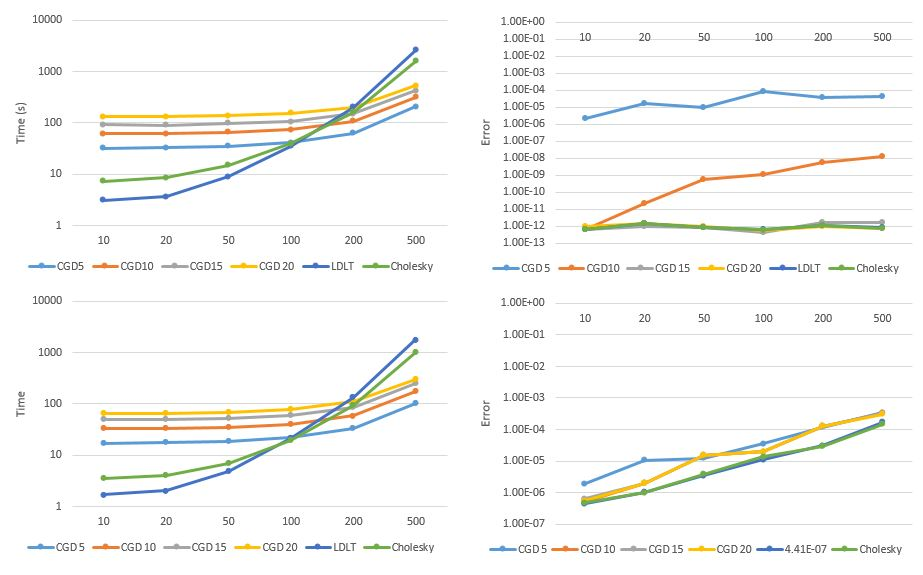
\includegraphics[scale=0.47]{results1.jpg}
  \caption{(Left) Run time comparison in seconds as a function of input dimension. (Right) Accuracy as a function of the input dimensionality $d$. (Top) Fixed-point numbers with the $b = 80$ bits, with 60 in the fractional part. (Bottom) $b = 41$, with 28 in the fractional part}
  \label{fig:result2}
\end{figure}

\noindent
We also varied the size of $N$ to see the effect of how different numbers of entries changed the accuracy of the algorithm. We noticed that the condition number of the matrix varies inversely with the amount of data in the system. More data means smaller condition number and thus better accuracy.

\begin{figure}[h]
\centering
  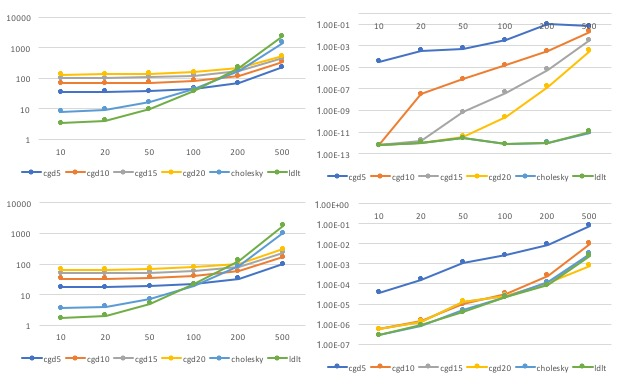
\includegraphics[scale=0.5]{results2.jpg}
  \caption{(Left) For N = 1000: Comparison between different methods of solving linear systems: running time in seconds for Cholesky, LDLT, and CGD as a function of input dimension. (Right) Accuracy of Cholesky, LDLT, and CGD, as a function of the input dimensionality $d$. (Top) Fixed-point numbers with the $b = 80$ bits, with 60 in the fractional part. (Bottom) $b = 41$, with 28 in the fractional part}
  \label{fig:result2}
\end{figure}  

\noindent
Secondly, we ran on a size 20 and size 100 matrices with varying condition numbers from 1 to 10. To replicate [1] we ran iterations of 5, 10, 15, and 20 for the CGD algorithm but also tried 25 iterations to see if there were improvements. 
\begin{figure}[H]
\centering
  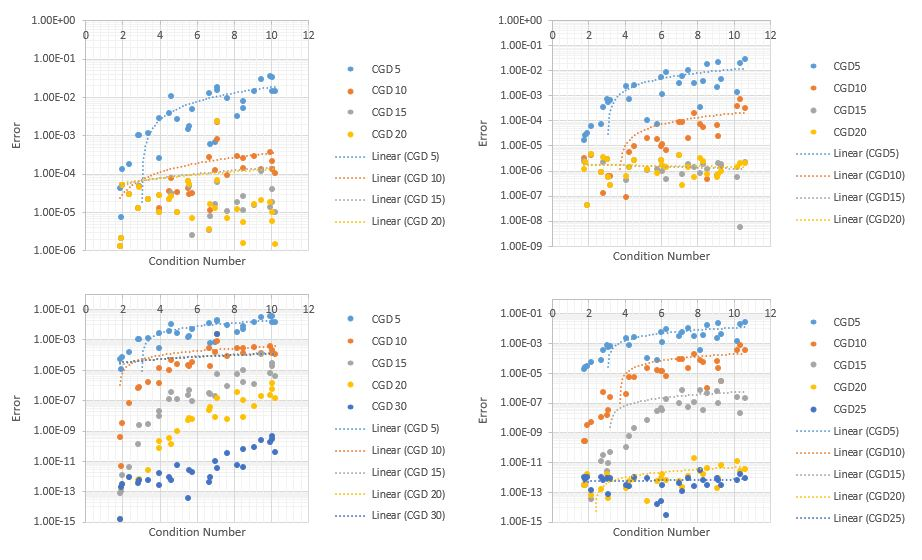
\includegraphics[scale=0.6]{conditionnumber.jpg}
  \caption{(Left) The plot of solving data with condition numbers ranging from 1 to 10 against the error, using matrices of size d = 100. (Right) The plot of solving data with condition numbers ranging from 1 to 10 against the error, using matrices of size d = 20. (Top) was ran in 32 bit SPDZ and (Bottom) was ran in 64 bit SPDZ.}
  \label{fig:result3}
\end{figure}

\noindent
In the condition number experiment, for CGD iterations of 5, 10, and 15, error increases as condition number increases. For example, in CGD 10 a small condition number may have an error of $\mathtt{10e-9}$ yet a larger condition number could have an error as large as $\mathtt{10e-3}$. However, in the CGD 20 case, the condition number does not have much effect due to the small errors, with the error varying only form $\mathtt{10e-11}$ to $\mathtt{10e-14}$. For the 60 bit precision case, we ran more iterations because there is a noticeable upward slope in the scatter plot in the CGD 20 line, indicating that still as condition numbers increased, the errors were increasing as well. Indeed, 25 iterations showed some improvement as we can see a flatter trend.\\

\noindent
To fine tune the CGD and Cholesky algorithms to SPDZ, we experimented with different ways of approximating square roots, to see if one or the other had better runtime or smaller error. The Babylonian method involves iteratively dividing and averaging an initial guess so on the next iteration can be represented as $x_{n+1} = \frac{1}{2} (x_{n} + \frac{S}{x_{n}})$. The Newton Method is similar but finds the square root using multiplications and not divisions: $\sqrt{S} = S \cdot (1/\sqrt{S})$. We originally hypothesized that using more multiplications over divisions should result in faster results. The results presented here are run on the Cholesky algorithm. However, since multiplication and division are implemented similarly in SPDZ, we did not find these results to be significant.

\begin{figure}[h]
     \centering
  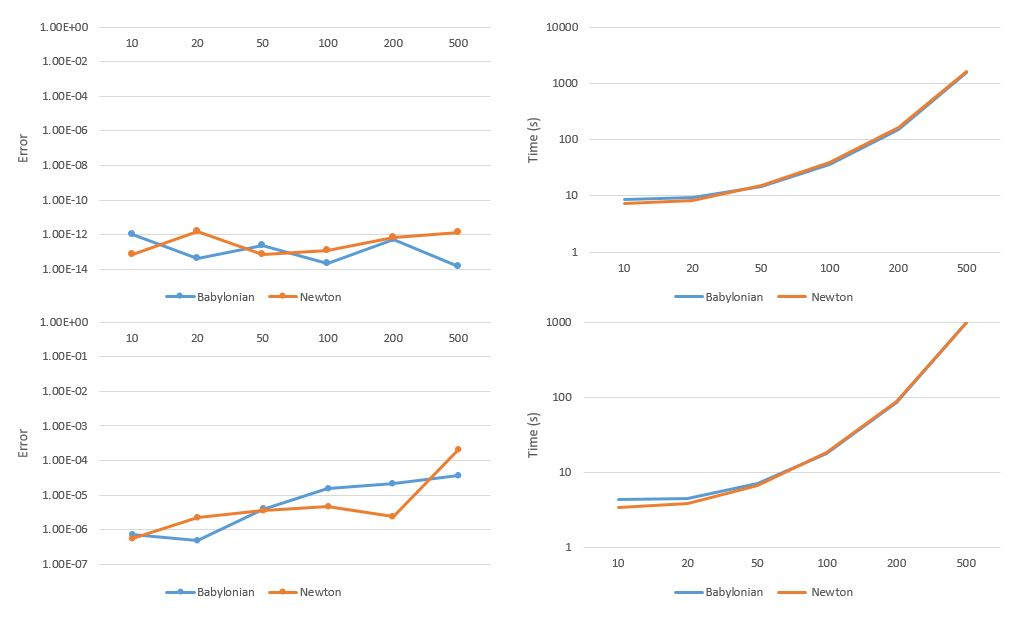
\includegraphics[scale=0.45]{sqrt.jpg}
  \caption{ 64 bit (top) and 32 bit (bottom) results for comparing approximating square roots methods.}
  \label{fig:result1}
\end{figure}

\noindent
For CGD, we decide to test if utilizing L2 norm vs Linfinity would make a difference in the algorithm. One utilizes comparisons which could be costly for arithmetic circuits and the other addition and square root. 

\begin{figure}[H]
\centering
  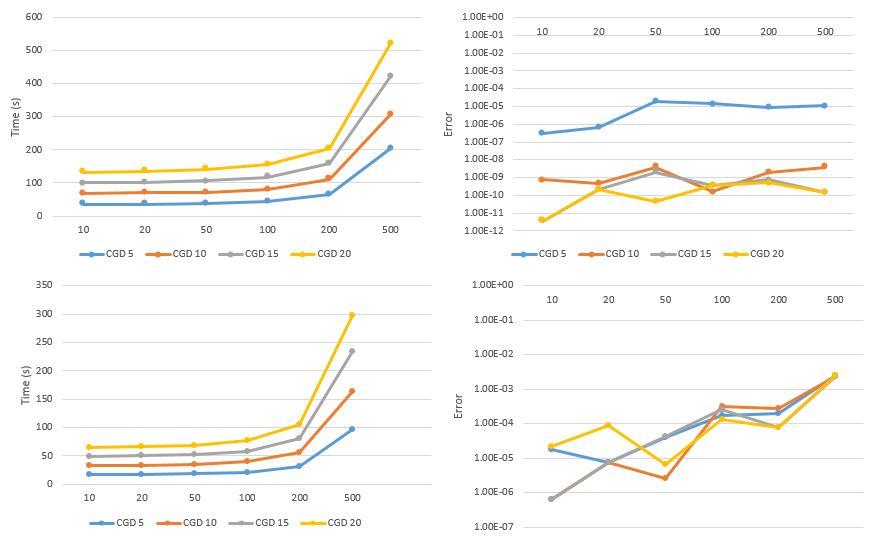
\includegraphics[scale=0.45]{l2.jpg}
  \caption{ (Top) 64 bit (Bottom) 32 bit results for L2 Norm. }
  \label{fig:result1}
\end{figure}

\subsection{Experiments on multiple parties and machines}

We also ran results for 3 and 4 players, which is also something that [1] considered. In a typical real world setting, there are often more than 2 parties, so we wanted to gauge what the additional run time would be for SPDZ to handle more parties. The error results were the same as those presented prior so we chose not to include them again. 

\begin{figure}[h]
\centering
  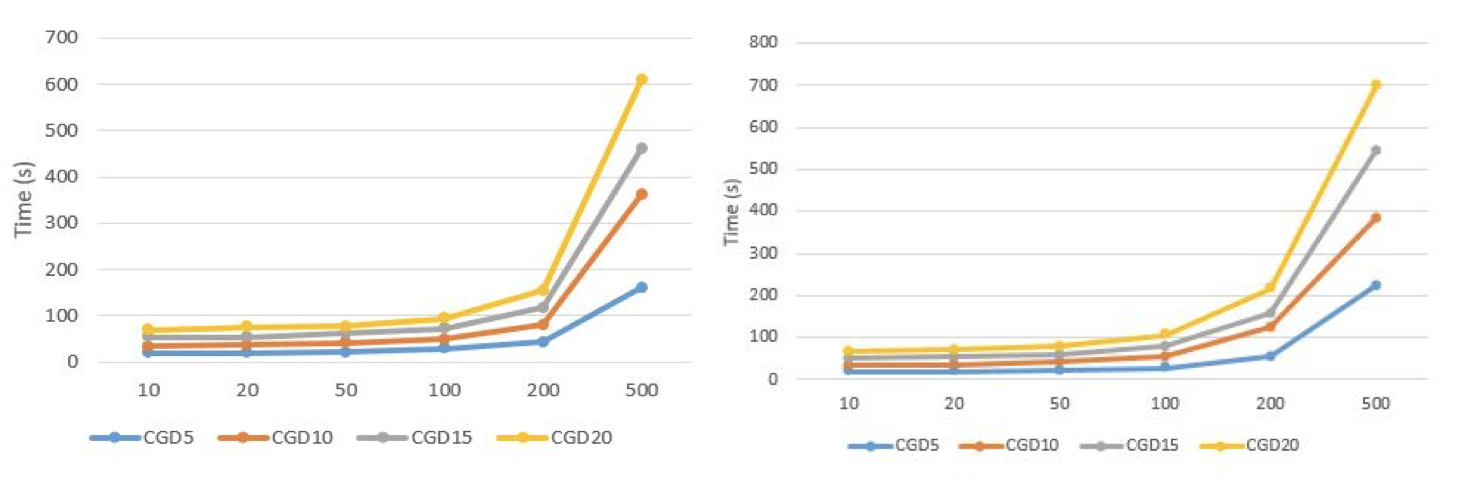
\includegraphics[scale=0.6]{multi.jpg}
  \caption{Run time results for 3 and 4 players in 32 bits. (Left) 3 Players. (Right) 4 Players.}
  \label{fig:result4}
\end{figure}

\noindent
Additionally, we deployed two Amazon EC2 instances of the c4.8xlarge type and performed the same experiments as before to gauge the latency of having two players on separate machines. The errors were the same as before, but we observed a drastic increase in run time over a network, compared to the previous two player results. 

\begin{figure}[h]
\centering
  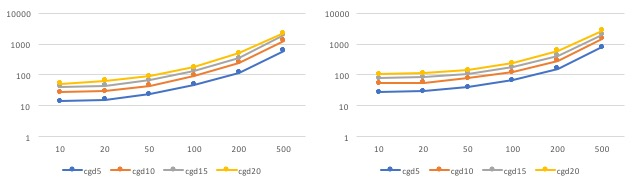
\includegraphics[scale=0.7]{ec2.jpg}
  \caption{Run time results for 2 players deployed on EC2 instances averaged over 15 runs. (Left) 32 bits. (Right) 64 bits.}
  \label{fig:result4}
\end{figure}

\subsection{Stochastic Gradient Descent}

To implement SGD, we utilized the update function presented in [2]: $ w = w - \frac{1}{|B|} \alpha X^{T}_{B} \times (X_{B} \times w - Y_{B})$. The first dataset that we worked with was MNIST. However, per [2], we only trained and tested on the 0s and 1s in the dataset. From Figure 8, we can observe that 13 bits are sufficient enough to achieve almost perfect accuracy for prediction.

\begin{figure}[H]
\centering
  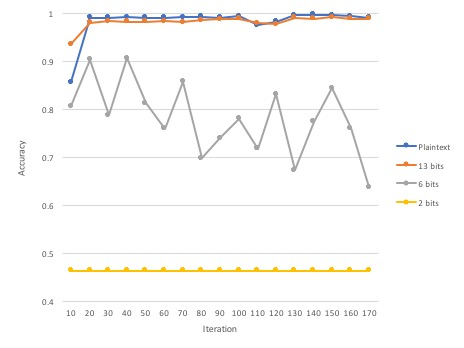
\includegraphics[scale=0.6]{mnist.jpg}
  \caption{Varying number of bits and recreating results in [2].}
  \label{fig:result4}
\end{figure}

\vc{Run these same results on Arcene dataset too}

\noindent
\\Using the same SGD algorithm, we also compared the resulting root mean squared error (RMSE) in 7 open sourced datasets of ranging sizes.

\begin{table}[H]
\centering
\label{my-label}
\begin{tabular}{@{}llllll@{}}
\toprule
Dataset Name          & \multicolumn{1}{c}{SGD Plaintext} & \multicolumn{2}{c}{\begin{tabular}[c]{@{}c@{}}SPDZ (28 bit)\\ error / time\end{tabular}} & \multicolumn{2}{c}{\begin{tabular}[c]{@{}c@{}}SPDZ (13 bit)\\ error / time\end{tabular}} \\ \midrule
Student Performance   & 0.11                              & 0.12 (+8.34\%)                                  & 2.174                                  & 0.12(+8.34\%)                                   & 2.616                                  \\
Auto MPG              & 0.56                              & 0.68 (+21.4\%)                                  & 0.663                                  & 0.68(+21.4\%)                                   & 0.704                                  \\
Communities and Crime & 0.06                              & 0.17 (+183\%)                                   & 10.352                                 & 0.19 (+216\%)                                   & 12.363                                 \\
Wine Quality          & 0.18                              & 0.19 (+5.55\%)                                  & 0.809                                  & 0.19 (+5.55\%)                                  & 0.969                                  \\
Bike Sharing          & 0.23                              & 0.24 (+4.34\%)                                  & 0.910                                  & 0.25 (+8.69\%)                                  & 1.097                                  \\
Year Prediction MSD   & 0.06                              & 0.06 (+0.0\%)                                   & 7.146                                  & 0.06 (+0.0\%)                                   & 8.513                                  \\
Gas Sensor Array      & 0.20                              & 0.36 (+20.0\%)                                  & 1.151                                  & 0.36 (+20.0\%)                                  & 1.559                                  \\ \bottomrule
\end{tabular}\\
\caption{SGD Results for 7 open sourced UCI datasets.}
\end{table}

\noindent
Running the results in a secure setting increased the RMSE in quite a few of the datasets, however it is important to note that even the increase is still quite low for large data sets. In comparison to CGD and Cholesky results from [1], SGD had lower RMSE even when run in SPDZ. 

\subsection{Analysis}

\begin{table}[H]
\centering
\label{my-label}
\begin{tabular}{@{}llll@{}}
\toprule
iterations & one machine      & two EC2      & {[}1{]} results    \\ \midrule
5     & 206.08 & 784.74  & 10,474.57 \\
10    & 313.07 & 1505.08 & 20,888.35 \\
15    & 418.69 & 2039.39 & 31,300.94 \\
20    & 527.28 & 2701.99 & n/a        \\ \bottomrule
\end{tabular}
\caption{Runtime comparison of SPDZ for CGD on one and two machines against [1] in seconds}
\end{table}

\noindent
The run times for SPDZ are always comparable if not much faster. In terms of run-time, we observe that both Cholesky and LDLT were faster for smaller dimensions when $d \leq 100$ and CGD is faster for larger dimensions when $d > 100$. This is consistent with the findings in the original experiment. For dimensions 100 and smaller, when Cholesky and LDLT are faster, they comparative differences are not that big (LDLT with 1.6 seconds compared to CGD 20 with 60.89 seconds) when compared to the largest differences between the larger sizes (LDLT with 1747 seconds and CGD5 with 97 seconds). It is also important to note that the time differences between 32 and 64 bits are not that large- only blank percent more compared to the garbled circuits result where doubling the number of bits roughly increased time by an entire magnitude of 10.  \\

\noindent
The major takeaways are that increasing the size of the matrix and increasing the condition number results in higher errors. To get better results, we need to run more iterations of CGD. For high condition numbers in large matrices, Cholesky and LDLT outperform the other methods. However, CGD does well in low condition numbers. 

\section{References}

\vc{will fix this later with bibtex}

[1] Privacy-Preserving Distributed Linear Regression on High-Dimensional Data

[2] SecureML

\end{document}